\documentclass[12pt, a4paper, oneside]{ctexart}
\usepackage{amsmath, amsthm, amssymb, bm, color, graphicx, geometry, mathrsfs,extarrows, braket, booktabs, array, wrapfig}
\usepackage[colorlinks,linkcolor=red,anchorcolor=blue,citecolor=blue,urlcolor=blue,menucolor=black]{hyperref}
\setCJKmainfont{方正新书宋_GBK.ttf}[ BoldFont = 方正小标宋_GBK, ItalicFont = 方正楷体_GBK]
\setmainfont{Times New Roman}  % 设置英文字体
\setsansfont{Calibri}
\setmonofont{Consolas}

\linespread{1.4}
%\geometry{left=2.54cm,right=2.54cm,top=3.18cm,bottom=3.18cm}
\geometry{left=1.84cm,right=1.84cm,top=2.18cm,bottom=2.18cm}
\newcounter{problem}  % 问题序号计数器
\newenvironment{problem}[1][]{\stepcounter{problem}\par\noindent\textbf{题目\arabic{problem}. #1}}{\smallskip\par}
\newenvironment{solution}[1][]{\par\noindent\textbf{#1解答. }}{\smallskip\par}  % 可带一个参数表示题号\begin{solution}{题号}
\newenvironment{note}{\par\noindent\textbf{注记. }}{\smallskip\par}

%%%% 图片相对路径 %%%%
\graphicspath{{figure/}} % 当前目录下的figure文件夹, {../figure/}则是父目录的figure文件夹

\everymath{\displaystyle} % 默认全部行间公式
\DeclareMathOperator*\uplim{\overline{lim}} % 定义上极限 \uplim_{}
\DeclareMathOperator*\lowlim{\underline{lim}} % 定义下极限 \lowlim_{}
\let\leq=\leqslant % 将全部leq变为leqslant
\let\geq=\geqslant % geq同理

%%%% 一些宏定义 %%%%
\def\bd{\boldsymbol}        % 加粗(向量) boldsymbol
\def\disp{\displaystyle}    % 使用行间公式 displaystyle(默认)
\def\tsty{\textstyle}       % 使用行内公式 textstyle
\def\sign{\text{sign}}      % sign function
\def\wtd{\widetilde}        % 宽波浪线 widetilde
\def\R{\mathbb{R}}          % Real number
\def\N{\mathbb{N}}          % Natural number
\def\Z{\mathbb{Z}}          % Integer number
\def\Q{\mathbb{Q}}          % Rational number
\def\C{\mathbb{C}}          % Complex number
\def\K{\mathbb{K}}          % Number Field
\def\P{\mathbb{P}}          % Polynomial
\def\d{\mathrm{d}}          % differential operator
\def\e{\mathrm{e}}          % Euler's number
\def\i{\mathrm{i}}          % imaginary number
\def\re{\mathrm{Re}}        % Real part
\def\im{\mathrm{Im}}        % Imaginary part
\def\res{\mathrm{Res}}      % Residue
\def\ker{\mathrm{Ker}}      % Kernel
\def\L{\mathcal{L}}         % Loss function
\def\wdh{\widehat}          % 宽帽子 widehat
\def\ol{\overline}          % 上横线 overline
\def\ul{\underline}         % 下横线 underline
\def\add{\vspace{1ex}}      % 增加行间距
\def\del{\vspace{-1.5ex}}   % 减少行间距

%%%% 定理类环境的定义 %%%%
\newtheorem{theorem}{定理}

%%%% 基本信息 %%%%
\newcommand{\RQ}{\today} % 日期
\newcommand{\km}{泛函分析} % 科目
\newcommand{\bj}{强基数学002} % 班级
\newcommand{\xm}{吴天阳} % 姓名
\newcommand{\xh}{2204210460} % 学号

\begin{document}

%\pagestyle{empty}
\pagestyle{plain}
\vspace*{-15ex}
\centerline{\begin{tabular}{*5{c}}
    \parbox[t]{0.25\linewidth}{\begin{center}\textbf{日期}\\ \large \textcolor{blue}{\RQ}\end{center}} 
    & \parbox[t]{0.2\linewidth}{\begin{center}\textbf{科目}\\ \large \textcolor{blue}{\km}\end{center}}
    & \parbox[t]{0.2\linewidth}{\begin{center}\textbf{班级}\\ \large \textcolor{blue}{\bj}\end{center}}
    & \parbox[t]{0.1\linewidth}{\begin{center}\textbf{姓名}\\ \large \textcolor{blue}{\xm}\end{center}}
    & \parbox[t]{0.15\linewidth}{\begin{center}\textbf{学号}\\ \large \textcolor{blue}{\xh}\end{center}} \\ \hline
\end{tabular}}
\begin{center}
    \zihao{-3}\textbf{第七次作业}
\end{center}
\vspace{-0.2cm}
% 正文部分
\begin{problem}[(2.3.1)]
    设$X$为$B$空间,$X_0$是$X$的闭子空间. 映射$\varphi:X\to X/X_0$定义为$\varphi:x\mapsto[x],\ (\forall x\in X)$,其中$[X]$表示$x$的商类. 证明$\varphi$是开映射.
\end{problem}
\begin{proof}
    由开映射定理可知,只需证$X/X_0$是完备的. 令$\{[x_n]\}\subset X/X_0$是Cauchy列,则存在子列$\{[x_{n_k}]\}$使得$||[x_{n_{k+1}}]-[x_{n_k}]|| = ||[x_{n_{k+1}}-x_{n_k}]||\leq 1/2^k$,由商空间范数定义可知,$\forall \varepsilon > 0$,$\exists y_k\in X_0$使得$||x_{n_{k+1}}-x_{n_{k}}+y_k|| < ||[x_{n_{k+1}}-x_{n_{k}}]||+\varepsilon\leq 1/2^k+\varepsilon$,则$||x_{n_{k+1}}-x_{n_{k}}+y_k|| < 1/2^k$,于是$\sum_{k=1}^\infty ||x_{n_{k+1}}-x_{n_{k}}+y_k|| < \sum_{k=1}^\infty\frac{1}{2^k}=1$绝对收敛,由于$X$是完备的,则$\sum_{k=1}^\infty x_{n_{k+1}}-x_{n_{k}}+y_k$收敛,令部分和$\{x_{n_{k+1}}+\sum_{i=1}^ky_i\}$收敛到$x+y,\ x\in X, y\in X_0$,由$\varphi$的连续性可得$\lim_{n\to\infty}[x_n] = \lim_{n\to\infty}\left[x_{n_k}+\sum_{i=1}^{k-1}y_i\right] = [x+y] = [x]\in X/X_0$,所以$X/X_0$是商空间.
\end{proof}
\begin{problem}[(2.3.2)]
    设$X,Y$是$B$空间,又设方程$Ux=y$对$\forall y\in Y$有解$x\in X$,其中$U\in L(X,Y)$,并且$\exists m  > 0$,使得$||Ux|| \geq m||x||,\ (\forall x\in X)$,求证:$U$有连续逆$U^{-1}$,并且$||U^{-1}||\leq 1/m$.
\end{problem}
\begin{proof}
    由条件可知$U$是满射,假设$\exists x_1,x_2\in X$使得$Ux_1=Ux_2$,则$U(x_1-x_2) = \theta\Rightarrow x_1=x_2$,于是$U$是单射,故$U$是双射.

    由逆算子定理可知$U^{-1}\in L(Y,X)$,由于$||Ux||\geq m||x||$,令$x = U^{-1}y$得$||y||\geq m||U^{-1}y||$,则$||U^{-1}y||\leq ||y||/m,\ (\forall y\in Y)$,则$||U^{-1}||\leq 1/m$.
\end{proof}
\begin{problem}[(2.3.3)]
    设$H$为Hilbert空间,$A\in L(H)$,且$\exists m > 0$,使得$|(Ax,x)|\geq m||x||^2,\ (\forall x\in H)$. 求证:$\exists A^{-1}\in L(H)$.
\end{problem}
\begin{proof}
    由逆算子定理知,只需证$A$为双射. 假设$\exists y_1,y_2\in X$使得$Ay_1=Ay_2$则
    \begin{equation*}
        m||y_1-y_2||^2\leq |(A(y_1-y_2),y_1-y_2)| = |(\theta,(y_1-y_2))| = 0\Rightarrow y_1=y_2
    \end{equation*}
    故$A$是单射. 
    
    下证$R(A)=Y$,只需证$R(A)$是闭的且$R(A)^\perp = \{\theta\}$. 设$\{Ax_n\}\subset H$收敛于$y\in H$,由于
    \begin{equation*}
        m||x||^2\leq |(Ax,x)|\leq ||Ax||\cdot||x||\Rightarrow m||x||\leq ||Ax||
    \end{equation*}
    于是$||x_{n+p}-x_n||\leq ||Ax_{n+p}-Ax_n||\to 0,\ (n\to\infty,\forall p>0)$则$\{x_n\}$为Cauchy列,由于$H$完备,令其收敛于$x$,由$A$的连续性可得$Ax=y\in R(A)$,所以$A$是闭的. 令$x_0\in R(A)^\perp$则$||x_0||^2\leq ||(Ax_0,x_0)||/m = 0\Rightarrow x_0 = \theta$则$\R(A)^\perp = \{\theta\}$,于是$\overline{R(A)} = R(A) = Y$. 所以$A$是满射.

    综上,$A$是双射.
\end{proof}
\begin{problem}[(2.3.4)]
    设$X,Y$是$B^*$空间,$D$是$X$的线性子空间,且$A:D\to Y$是线性映射. 求证:
    
    (1). 若$A$连续且$D$是闭的,则$A$是闭算子.

    (2). 若$A$连续且是闭算子,则$Y$完备蕴含$D$是闭的.

    (3). 若$A$是单射的闭算子,则$A^{-1}$也是闭算子.

    (4). 若$X$完备,$A$是单射的闭算子,$R(A)$在$Y$中稠密,且$A^{-1}$连续,那么$R(A) = Y$.
\end{problem}
\begin{proof}
    (1). $\forall \{x_n\}\subset D$满足$x_n\to x,\ Ax_n\to y$,由于$D$是闭的可得$x\in D$,由$A$连续性可得$Ax_n\to Ax = y$,所以$A$是闭算子.

    (2). 反设$D$是开的,则$\exists x_0\in X\setminus D,\ \{x_n\}\subset D$使得$x_n\to x_0$,由于
    \begin{equation*}
        ||Ax_{n+p}-Ax_n||\leq ||A||\cdot ||x_{n+p}-x_n||\to 0,\ (n\to\infty,\ \forall p > 0)
    \end{equation*}
    则$\{Ax_n\}$是$Y$中的Cauchy列,令$\lim_{n\to\infty}Ax_n = y$,由于$A$为闭算子,则$x\in D$,这与$x\in X\setminus D$矛盾. 故$D$是闭的.

    (3). 由于$A$是单射,则$A^{-1}$有意义,$\forall \{y_n\}\subset R(A)$满足$y_n\to y,\ A^{-1}y_n\to x$,由$A$是闭算子,则$A^{-1}y_n\to A^{-1}y,\ y_n\to Ax$可得到$A^{-1}y\in D$且$A(A^{-1}y)=y=Ax$,于是$y\in R(A)$且$A^{-1}y\in X$.

    (4). 由(3)可知,$A^{-1}$是闭算子,由(2)可知$X$完备且$A^{-1}$连续,则$R(A)$是闭的,又由于$R(A)$在$Y$中稠密,则$R(A) = \ol{R(A)} = Y$.
\end{proof}
% 下面给一些功能的写法
\iffalse
% 图片模板
\centerline{
    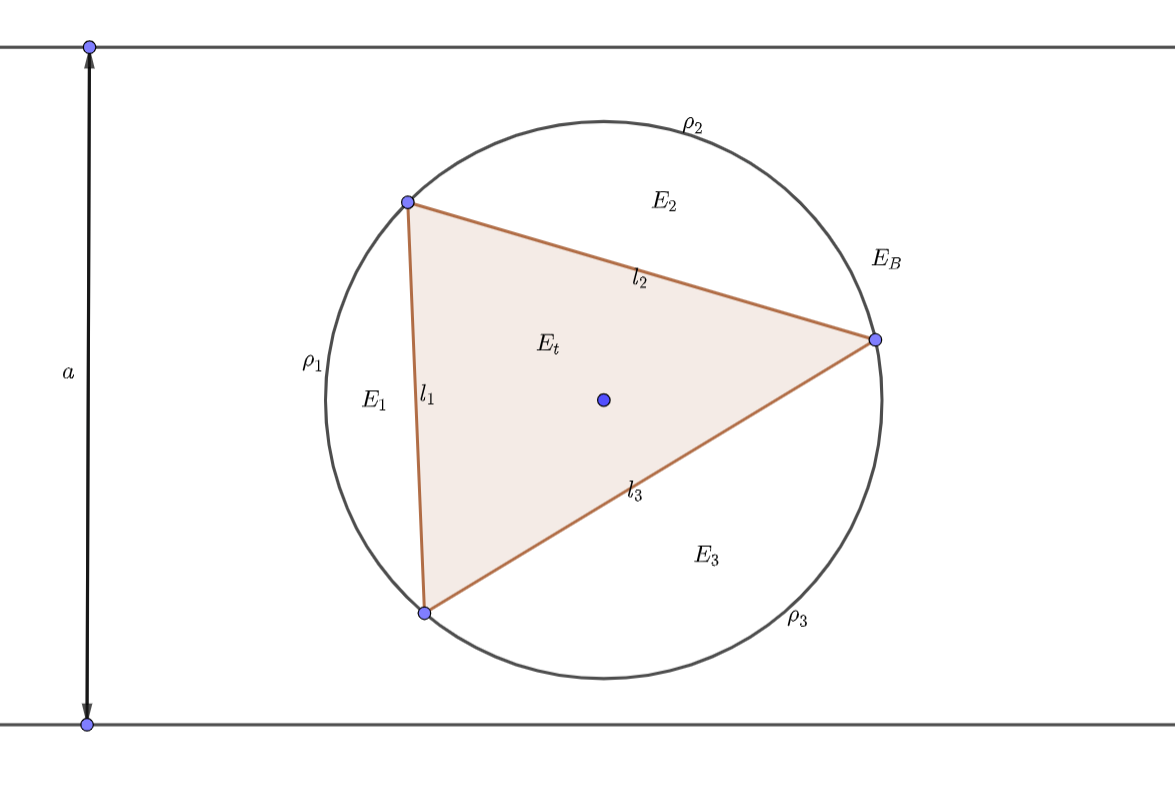
\includegraphics[width=0.8\textwidth]{figure.png}
}
% 表格模板
\renewcommand\arraystretch{0.8} % 设置表格高度为原来的0.8倍
\begin{table}[!htbp] % table标准
    \centering % 表格居中
    \begin{tabular}{p{1cm}<{\centering}p{1cm}<{\centering}p{3cm}<{\centering}p{5cm}<{\centering}} % 设置表格宽度
    %\begin{tabular}{cccc}
        \toprule
        $x_i$ & $f[x_1]$ & $f[x_i,x_{i+1}]$ & $f[x_i,x_{i+1},x_{i+2}]$ \\
        \midrule
        $x_0$ & $f(x_0)$ &                  &                          \\
        $x_0$ & $f(x_0)$ & $f'(x_0)$        &                          \\
        $x_0$ & $f(x_1)$ & $\frac{f(x_1)-f(x_0)}{x_1-x_0}$ & $\frac{f(x_1)-f(x_0)}{(x_1-x_0)^2}-\frac{f'(x_0)}{x_1-x_0}$\\
        \bottomrule
    \end{tabular}
\end{table}

\def\Log{\text{Log}} % 一个简单的宏定义
$\Log$ % 调用方法
\fi

\end{document}